% Source for docs/static/img/reinforce-training.svg. Rebuild from the repository root:
%   pdflatex -output-directory=/tmp docs/scripts/reinforce-training.tex
%   pdf2svg /tmp/reinforce-training.pdf docs/static/img/reinforce-training.svg
%   python3 docs/scripts/prepare_rollout_svgs.py
\documentclass[tikz,border=3pt]{standalone}
\usepackage{amsmath,amssymb,bm}
\usetikzlibrary{arrows.meta,positioning,calc,fit}

\colorlet{agentA}{red!80!black}     % agent 1: policy, prompts, responses, loss
\colorlet{agentB}{blue!80!black}    % agent 2
\colorlet{learned}{orange!80!black} % learned evaluators: critic, reward model
\colorlet{update}{green!50!black}   % gradients and parameter updates

\tikzset{
  >={Stealth[length=3.2pt,width=3pt]},
  box/.style={draw, line width=1pt, inner sep=2.5pt, minimum height=13pt},
  policy/.style={box, rounded corners=3pt, minimum width=30pt},
  flow/.style={->, line width=.8pt},
  note/.style={font=\scriptsize, align=left},
  label/.style={anchor=west, font=\footnotesize},
}

% One rollout node of the MAREINFORCE family (MAGRPO, MAREINFORCE, MARLOO, MAReMax).
% Columns: agent 1 (left), shared quantities (center), agent 2 (right).
\begin{document}
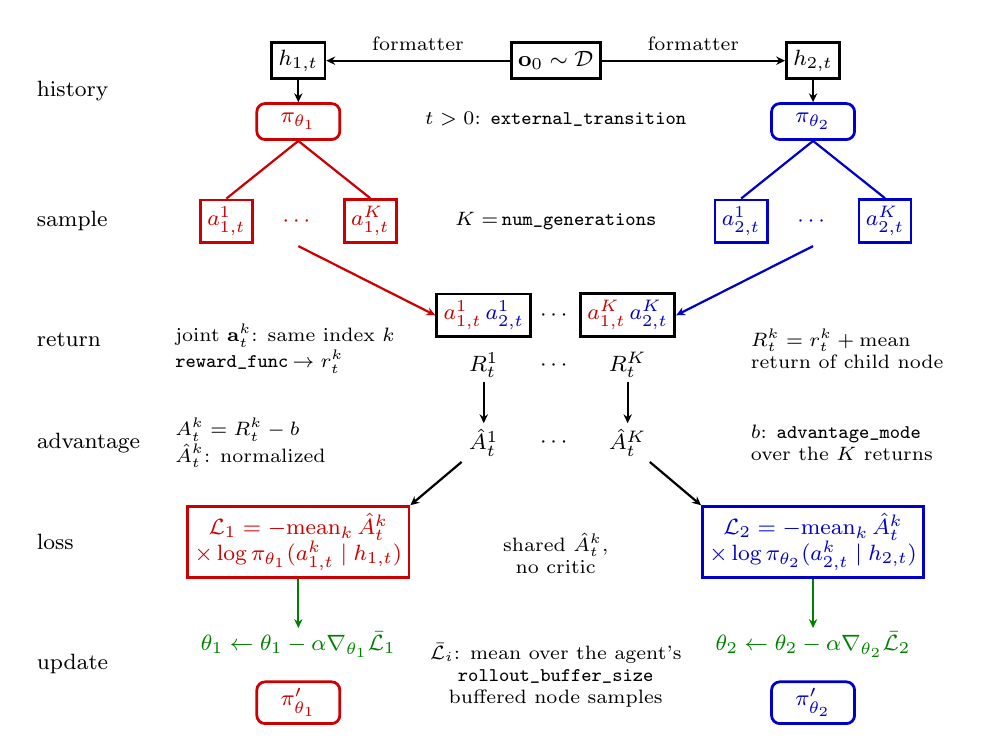
\begin{tikzpicture}[x=1pt, y=1pt, font=\footnotesize]
  \def\xa{98}   % agent 1 column
  \def\xc{191}  % shared column
  \def\xb{284}  % agent 2 column

  % Stage 0: task item, prompts and policies.
  \node[label] at (0,-11) {history};
  \node[box] (o) at (\xc,0) {$\mathbf{o}_0\sim\mathcal{D}$};
  \node[box] (h1) at (\xa,0) {$h_{1,t}$};
  \node[box] (h2) at (\xb,0) {$h_{2,t}$};
  \draw[flow] (o) -- node[above, font=\scriptsize] {formatter} (h1);
  \draw[flow] (o) -- node[above, font=\scriptsize] {formatter} (h2);
  \node[policy, agentA] (p1) at (\xa,-22) {$\pi_{\theta_1}$};
  \node[policy, agentB] (p2) at (\xb,-22) {$\pi_{\theta_2}$};
  \draw[flow] (h1) -- (p1);
  \draw[flow] (h2) -- (p2);
  \node[note] at (\xc,-21) {$t>0$: \texttt{external\char95transition}};

  % Stage 1: K responses per agent.
  \node[label] at (0,-58) {sample};
  \node[box, agentA] (a11) at (\xa-26,-58) {$a^{1}_{1,t}$};
  \node[agentA] at (\xa,-58) {$\cdots$};
  \node[box, agentA] (a1K) at (\xa+26,-58) {$a^{K}_{1,t}$};
  \node[box, agentB] (a21) at (\xb-26,-58) {$a^{1}_{2,t}$};
  \node[agentB] at (\xb,-58) {$\cdots$};
  \node[box, agentB] (a2K) at (\xb+26,-58) {$a^{K}_{2,t}$};
  \foreach \n in {a11,a1K} \draw[agentA, line width=.8pt] (p1.south) -- (\n.north);
  \foreach \n in {a21,a2K} \draw[agentB, line width=.8pt] (p2.south) -- (\n.north);
  \node[note] at (\xc,-58) {$K=$\,\texttt{num\char95generations}};

  % Stage 2: aligned joint responses and their shared returns.
  \node[label] at (0,-101) {return};
  \node[box] (j1) at (\xc-26,-92)
    {$\textcolor{agentA}{a^{1}_{1,t}}\,\textcolor{agentB}{a^{1}_{2,t}}$};
  \node at (\xc,-92) {$\cdots$};
  \node[box] (jK) at (\xc+26,-92)
    {$\textcolor{agentA}{a^{K}_{1,t}}\,\textcolor{agentB}{a^{K}_{2,t}}$};
  \draw[flow, agentA] (\xa,-67) -- (j1.west);
  \draw[flow, agentB] (\xb,-67) -- (jK.east);
  \node at (\xc-26,-110) {$R^{1}_t$};
  \node at (\xc,-110) {$\cdots$};
  \node at (\xc+26,-110) {$R^{K}_t$};
  \node[note, anchor=west] at (50,-104) {joint $\mathbf{a}^k_t$: same index $k$\\\texttt{reward\char95func}$\,\to r^k_t$};
  \node[note, anchor=west] at (258,-104) {$R^k_t=r^k_t+{}$mean\\return of child node};

  % Stage 3: shared group-relative advantages.
  \node[label] at (0,-138) {advantage};
  \draw[flow] (\xc-26,-116) -- (\xc-26,-131);
  \draw[flow] (\xc+26,-116) -- (\xc+26,-131);
  \node at (\xc-26,-138) {$\hat A^{1}_t$};
  \node at (\xc,-138) {$\cdots$};
  \node at (\xc+26,-138) {$\hat A^{K}_t$};
  \node[note, anchor=west] at (50,-138) {$A^k_t=R^k_t-b$\\$\hat A^k_t$: normalized};
  \node[note, anchor=west] at (258,-138) {$b$: \texttt{advantage\char95mode}\\over the $K$ returns};

  % Stage 4: per-agent losses weighted by the shared advantages.
  \node[label] at (0,-174) {loss};
  \node[box, agentA, align=center] (l1) at (\xa,-174)
    {$\mathcal{L}_1=-\mathrm{mean}_k\,\hat A^k_t$\\$\times\log\pi_{\theta_1}(a^k_{1,t}\mid h_{1,t})$};
  \node[box, agentB, align=center] (l2) at (\xb,-174)
    {$\mathcal{L}_2=-\mathrm{mean}_k\,\hat A^k_t$\\$\times\log\pi_{\theta_2}(a^k_{2,t}\mid h_{2,t})$};
  \draw[flow] (\xc-34,-145) -- (l1.north east);
  \draw[flow] (\xc+34,-145) -- (l2.north west);
  \node[note, align=center] at (\xc,-178) {shared $\hat A^k_t$,\\no critic};

  % Stage 5: buffered per-agent optimizer steps.
  \node[label] at (0,-218) {update};
  \draw[flow, update] (l1.south) -- (\xa,-205);
  \draw[flow, update] (l2.south) -- (\xb,-205);
  \node[update] (u1) at (\xa,-211) {$\theta_1\leftarrow\theta_1-\alpha\nabla_{\theta_1}\bar{\mathcal{L}}_1$};
  \node[update] (u2) at (\xb,-211) {$\theta_2\leftarrow\theta_2-\alpha\nabla_{\theta_2}\bar{\mathcal{L}}_2$};
  \node[policy, agentA] at (\xa,-232) {$\pi_{\theta_1}'$};
  \node[policy, agentB] at (\xb,-232) {$\pi_{\theta_2}'$};
  \node[note, align=center] at (\xc,-222) {$\bar{\mathcal{L}}_i$: mean over the agent's\\\texttt{rollout\char95buffer\char95size}\\buffered node samples};
\end{tikzpicture}
\end{document}
